\chapter{Entanglement amplification via the Unruh-Hawking effect\footnote{M. Montero and E. Mart\'in-Mart\'inez. arXiv:1011.6540}}\label{generatio}


We have studied in previous chapters the influence of the so-called Unruh and Hawking effects on quantum entanglement. In all these previous studies it was shown how starting with entangled states from an inertial perspective we end up with a less entangled state when one of the observers is non-inertial. Due to those results, it has been always considered that the Unruh effect would only be able to degrade entanglement.

This belief was reinforced by the intuitive argument that since the Unruh effect acts in a similar way to a thermal bath with $T\propto a$,  entanglement should be degraded in a similar way as by thermal decoherence. This argument is flawed because the Unruh thermal state is derived for the Minkowski vaccuum state, not for states containing excitations. Nevertheless, it was supported  by the fact that all previous works under the single mode approximation (SMA) found that entanglement in the AR bipartition was a monotonically decreasing function of the acceleration. Also, for maximally entangled states beyond the SMA, the same monotonic behaviour of AR entanglement was found (see figures \ref{figbosons} and \ref{bundlefm7}). So it still seemed true that acceleration tends to degrade entanglement. When studying non-maximally entangled states these trends would be expected to continue holding in principle.

In this chapter we show an unexpected outcome of the Unruh and Hawking effects: the appearance of entanglement when one of the observers of a bipartite system undergoes a constant acceleration. We prove here that there are some states, shared by two observers, whose degree of entanglement increases as one of the observers accelerates. The phenomenon is thoroughly studied here for Grassmann scalar and bosonic scalar fields, it is thus not a peculiarity of fermionic statistics (as it was the entanglement survival in the infinite acceleration limit) but a universal phenomenon. 

This entanglement amplification is promising in order to detect quantum effects due to acceleration (and therefore gravity). Entanglement, unlike other phenomena (such as thermal noise) does not admit a classical description. Thus, its observation would account for a pure quantum origin of the aforementioned effects. 

On the other hand entanglement is very sensitive to any interaction with the environment, which tends to degrade it. This made it very difficult for any experiment relying on entanglement degradation \cite{Alicefalls} to find evidence for these effects. By the same token, experiments studying entanglement creation are safer from these flaws: if a small amount of entanglement is created, no matter how damped by decoherence it may be, the only possible origin is an acceleration-induced quantum effect. The entanglement amplification phenomenon provides a novel way to distinguish genuine quantum effects of gravity from classically induced ones, something worth considering when trying to detect the Unruh and Hawking effects in analog gravity set-ups \cite{garay}.  

The main reason why this phenomenon has gone unnoticed so far is the reliance in the single mode approximation (SMA)  that many previous works assumed. And, on the other hand when going beyond the single mode approximation, only maximally entangled states were studied. We need to study non-maximally entangled states beyond SMA to find the effect.


\section{The setting}

Let us consider a system composed of an inertial observer, Alice, who watches an inertial mode of a quantum field (either a Grassmann or bosonic scalar  field) and a uniformly accelerated Rindler observer either in region I or II of Rindler spacetime. As in previous chapters we will call this observer Rob if he is in region I and AntiRob if he is in region II. Rob (or AntiRob) watches an Unruh mode of the quantum field (see chapter \ref{sma}), which is entangled with Alice's. As we saw in chapter \ref{sma}, consideration of two different kinds of Unruh modes is necessary for a complete description of an arbitrary solution to the field equation.

 We will only consider Unruh modes of a given Rindler frequency $\omega$ as seen by Rob or AntiRob (who moves with proper acceleration $a$) but which are arbitrary superpositions of left and right mover modes, so that the creation and annihilation operators that we are considering here are  of the general form \eqref{eq:q-defs} for a scalar field and \eqref{creat} for the Grassmann scalar field. This is to say
 \begin{align}C_\omega=q_\text{L}C_{\omega,\text{L}}+\qr C_{\omega,\text{R}}\label{umodes},\end{align}
where $\vert q_\text{L}\vert^2+\vert\qr\vert^2=1$, $\qr \ge q_\text{L}$ and $C_{\omega,X}$ for $X=\text{L},\text{R}$ are
\begin{eqnarray}\label{bogoboson}
 C_{\omega,\text{R}}&=&\cosh r_{\text{b},\omega}\, a_{\omega,\text{I}} - \sinh r_{\text{b},\omega}\, a^\dagger_{\omega,\text{II}},\\*
 C_{\omega,\text{L}}&=&\cosh r_{\text{b},\omega}\, a_{\omega,\text{II}} - \sinh r_{\text{b},\omega}\, a^\dagger_{\omega,\text{I}}, \end{eqnarray}
where $a,a^\dagger$ are particle operators for the scalar field, and
\begin{eqnarray}\label{Unruhop}
\nonumber C_{\omega,\text{\text{R}}}&=&\left(\cos r_{\text{f},\omega}\, c_{\omega,\text{I}}-\sin r_{\text{f},\omega}\, d^\dagger_{\omega,\text{II}}\right),\\*
C_{\omega,\text{\text{L}}}&=&\left(\cos r_{\text{f},\omega}\, c_{\omega,\text{II}}-\sin r_{\text{f},\omega}\, d^\dagger_{\omega,\text{I}}\right),
\end{eqnarray}
where $c,c^\dagger$ and $d,d^\dagger$ are respectively particle and antiparticle operators, for the Grassmann case.

The family of bipartite states in which we will observe entanglament amplification is of the form 
\begin{align}\label{geGras} \ket{\Psi}&= P \ket{0}_\text{A} \left[\alpha\ket{1} +\sqrt{1-\alpha^2}\ket{0}\right] + \sqrt{1-P^2}\ket{1}_\text{A} \left[\beta\ket{1}+ \sqrt{1-\beta^2}\ket{0}\right]
.\end{align}
Here, the subscript `A' refers to Alice's inertial mode, and $\ket{1}=C^\dagger_\omega\ket{0}$ is the Unruh particle excitation. All these states have an implicit dependence on Rob's acceleration $a$ when expressed in the Rindler basis through the parameter defined by $\tan r_{\text{f},\omega}=e^{-\pi c\,\omega/a}$ in the fermionic case, and $\tanh r_{\text{b},\omega}=e^{-\pi c\,\omega/a}$ in the bosonic case.

As usual \cite{Alicefalls,AlsingSchul}, we transform the state \eqref{geGras} into the Rindler basis following the same conventions as in chapter \ref{sma}. Although the system is obviously bipartite, shifting to the Rindler basis for the second qubit the mathematical description of the system admits a straightforward tripartition: Minkowskian modes, Rindler region I modes, and Rindler region II  modes. 

The density matrix for the state, which includes modes on both wedges of the spacetime along with Minkowskian modes, is built from \eqref{geGras}. Namely, $\rho^{\text{AR}\bar{\text{R}}}=\proj{\Psi}{\Psi}$.

As discussed previously, an accelerated observer in region I is causally disconnected from region II (and vice-versa). For this reason when we consider the bipartite system Alice-Rob we need to trace over the modes that only have support in region II and to which Rob is causally disconnected. Equivalently, we would have to trace over modes in region I if we consider that the accelerated observer is in region II. The density matrices for the bipartite systems Alice-Accelerated observer are 
\begin{align}
\label{AR2}\rho^{\text{AR}}&=\tr_{\text{II}}\rho^{\text{AR}\bar{\text{R}}}=\sum_{n} \bra{n}_{\text{II}}\rho^{\text{AR}\bar{\text{R}}}\ket{n}_{\text{II}},\\*
\label{AAR2}\rho^{\text{A}\bar{\text{R}}}&=\tr_{\text{I}}\rho^{\text{AR}\bar{\text{R}}}=\sum_{n} \bra{n}_{\text{I}}\rho^{\text{AR}\bar{\text{R}}}\ket{n}_{\text{I}}.
\end{align}

The density matrix for the subsystem Alice-Rob is, therefore, given by
\begin{align}\label{rhog}\rho^{\text{A}{\text{R}}}&=\tr_\text{II}(\ket{\Psi}\bra{\Psi})=P^2\ket{0}_\text{A}\bra{0}_\text{A}\left[\alpha^2\tr_\text{II}(\ket{1}_\text{U}\bra{1}_\text{U})\right.+(1-\alpha^2)\tr_\text{II}(\ket{0}\bra{0})\nonumber\\&\!+\!\left.\alpha\sqrt{1\!-\!\alpha^2}\left(\tr_\text{II}(\ket{1}_\text{U}\bra{0})\!+\!\tr_\text{II}(\ket{0}\bra{1}_\text{U})\right)\right]\!+\!(1\!-\!P^2)\ket{1}_\text{A}\bra{1}_\text{A}\left[\beta^2\tr_\text{II}(\ket{1}_\text{U}\bra{1}_\text{U})\right.\nonumber\\&+(1-\beta^2)\tr_\text{II}(\ket{0}\bra{0})+\left.\beta\sqrt{1-\beta^2}\left(\tr_\text{II}(\ket{1}_\text{U}\bra{0})+\tr_\text{II}(\ket{0}\bra{1}_\text{U})\right)\right]\nonumber\\&+P\sqrt{1-P^2}\ket{1}_\text{A}\bra{0}_\text{A}\left[\alpha\beta\tr_\text{II}(\ket{1}_\text{U}\bra{1}_\text{U})\right.+\sqrt{1-\alpha^2}\sqrt{1-\beta^2}\tr_\text{II}(\ket{0}\bra{0})\nonumber\\&+\left.\beta\sqrt{1-\alpha^2}\tr_\text{II}(\ket{1}_\text{U}\bra{0})\right.\left.\alpha\sqrt{1-\beta^2}\tr_\text{II}(\ket{0}\bra{1}_\text{U})\right]+(\text{H.c.})_\text{Alice-Nondiag}\end{align}
for both cases, scalar field and Grassmann field. The kets and bras labeled with an A correspond to Alice and those inside the traces correspond to Rob.  by $(\text{H.c.})_\text{Alice-Nondiag}$ we mean the Hermitian conjugate of the terms with different Alice indices. 

The relevant matrices in \eq{rhog} are different for the scalar and the Grassmann case. Specifically, for the Grassmann scalar case
\begin{align}\tr_\text{II}(\ket{0}\bra{0})&=C^4\proj{00}{00}+S^2C^2(\proj{10}{10}+\proj{01}{01})+S^4\proj{11}{11},\nonumber\\\tr_\text{II}(\ket{1}_\text{U}\bra{1}_\text{U})&=\qr^2\left[C^2\proj{10}{10}+S^2\proj{11}{11}\right]+\ql^2\left[S^2\proj{10}{10}+C^2\proj{00}{00}\right]\nonumber\\
&-\qr\ql SC(\proj{11}{00}+\proj{00}{11}),\end{align}
and
\begin{align}\tr_\text{II}(\ket{1}_\text{U}\bra{0})&=\qr\left[C^3\proj{10}{00}+S^2C\proj{11}{01}\right]-\ql\left[S^3\proj{10}{11}+SC^2\proj{00}{01}\right].\end{align}
Where we have defined for brevity $S\equiv\sin r_{\text{f},\omega}$, $C\equiv\cos{\text{f},\omega}$ and $\ket{ij}$ is a state with $i$ particles and $j$ antiparticles in region I, obtained after tracing out the modes in region II.

The partial transpose with respect to Alice can be obtained by simply swapping the Alice states in \eq{rhog}. The resultant matrix can be diagonalised numerically to compute the negativity.

We shall now compute the density matrix after tracing out region II for the scalar field. For a general state \eqref{geGras} , the traced density matrix is given again by \eq{rhog}, but now the relevant matrices have a different form, namely
\begin{align}\nonumber\tr_\text{II}(\ket{0}\bra{0})&=\sum_{n=0}^\infty f(n)^2\proj{n}{n},\\\tr_\text{II}(\ket{1}_\text{U}\bra{1}_\text{U})&=\frac{1}{\cosh^2\ro}\sum_{n=0}^\infty f(n)^2(n+1)\left(\ql^2\proj{n}{n}+\qr^2\proj{n+1}{n+1}\right)\nonumber\\&+
\ql\qr f(n)f(n+1)\sqrt{(n+1)(n+2)}\left(\proj{n}{n+2}+\proj{n+2}{n}\right)\end{align}
and
\begin{align}\tr_\text{II}(\ket{1}_\text{U}\bra{0})&=\frac{1}{\cosh\ro}\sum_{n=0}^\infty \ql f(n)f(n+1)\sqrt{(n+1)}\proj{n}{n+1}\nonumber\\&+\qr f(n)^2\sqrt{n+1}\proj{n+1}{n}\end{align},
where $\ket{n}$ are field modes in region I and
\begin{equation}
f(n)=\frac{\tanh^n r_\Omega}{\cosh r_\Omega}.
\end{equation}
The resultant matrix is diagonalised numerically taking proper care of convergence issues to compute the negativity that we use to quantify the entanglement between Alice and Rob. Analogous operations would lead to Alice-AntiRob density matrix tracing over I instead of II as discussed in previous chapters (See for instance chapter \ref{sma}). 


\section{Entanglement amplification}

For $\qr\neq1$ and a rather simple choice of parameters in \eqref{geGras} (for instance, $P=0.4$, $\alpha=0$, $\beta=1$) the surprise appears: there can be entanglement amplification due to acceleration, as seen in fig. \ref{ent}. Furthermore, this amplification becomes more evident as $\qr$ approaches the extremal value $\qr=1/\sqrt{2}$.  AR and $\text{A}\bar{\text{R}}$ behave the same way in this case since the symmetry between regions I and II is not explicitly broken (see eq. \eqref{umodes} and chapter \ref{sma}). As $\qr$ tends to 1 (limit analogous to the SMA), the effect vanishes. 

More importantly, it is also possible to obtain high entanglement amplification considering almost separable states. In some of these cases the negativity is a increasing monotone function of $r_\omega$ (as for instance in \eqref{geGras} when $P=0.1$, $\alpha=0.8695$, $\beta=0.909$). Therefore, there are states for which the Unruh effect does exactly the opposite of what was expected. That is to say, entanglement is monotonically created rather than being monotonically destroyed.
\begin{figure}[h] 
\begin{center}
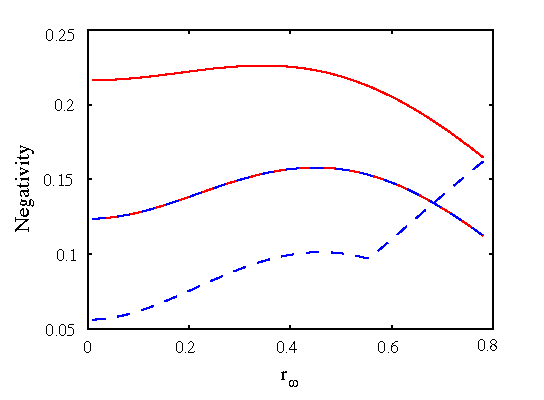
\includegraphics[width=.85\textwidth]{figabv5}
\end{center}
\caption{Entanglement amplification in Alice-Rob and Alice-AntiRob bipartitions for the Grassmann scalar field. Negativity curves for $AR$ (red continuous lines) and $A\bar R$ (blue dashed lines) as a function of $r_\omega$ for $\qr=0.85$ and $\qr=1/\sqrt{2}$ (where both contributions are equal). The state considered is of the general form \eqref{geGras}, with the choice of parameters $P=0.4$, $\alpha=0$, $\beta=1$. }
\label{ent}
\end{figure}

The phenomenon of entanglement creation also shows up for the bosonic scalar field, much in the same way as it did in the Grassmann case. The main difference is that  in the bosonic case entanglement is bound to vanish in the infinite acceleration limit, in concordance with previous results. Therefore, entanglement can be created only for a finite range of accelerations, as shown in Fig.\ref{ent2}. For $\qr=1/\sqrt{2}$, Alice-Rob negativity attains a maximum of $0.127$ at $r_\omega=0.191$. This is  3.1 \% above inertial level. Considering frequencies of order $\approx 1$  GHz, which correspond to reasonable experimental possibilities \cite{Adessada} the acceleration corresponding to this value of $r_\omega$ is $a\approx 10^{17}g$, much closer to experimental feasibility than previous proposals \cite{ChenTaj} which suggested accelerations of $\approx 10^{25}g$.


In order to study the experimental implications of this phenomenon, let us introduce a specific scenario. Consider the family of states \eq{geGras} for fixed $P$ and $\beta \gtrsim 0.2$. This family shows an unbounded relative increase of entanglement  as one approaches the limit $\alpha\rightarrow \beta$ (separable limit). This means that  there are states for which an arbitrary small acceleration produces an arbitrary large relative increase in negativity. The same happens as  we approach a separable state taking $P\rightarrow0$ for certain values of $\alpha$ and $\beta$. This behaviour is quite general and appears for both fermionic and bosonic fields. However the more relative entanglement increase (signal-to-background ratio) we want to achieve, the more separable the inertial states should be. Preparing and controlling these quasi-separable states would be the experimental challenge to detect the Unruh effect by means of these techniques.

Any such experiment would be naturally interested in negativity behaviour in the vicinity of $r_\omega=0$, easier to obtain in laboratory conditions. This means that in order to maximise experimental feasibility we are interested in states whose negativity shows a quick growth for small $r_\omega$. We study the relative increase of $AR$ negativity with respect to its inertial value for the family of states \eqref{geGras} at fixed $r_\omega$. As an example we choose  $r_\omega=0.15$ which corresponds to accelerations from $a\approx 5\cdot10^{13}g $ to $5\cdot10^{16} g$ for frequencies from $1 \text{ MHz}$ to $1 \text{ GHz}$. This unbounded entanglement creation can be seen in Fig. \ref{unbo}.

  \begin{figure}[h] 
  \begin{center}
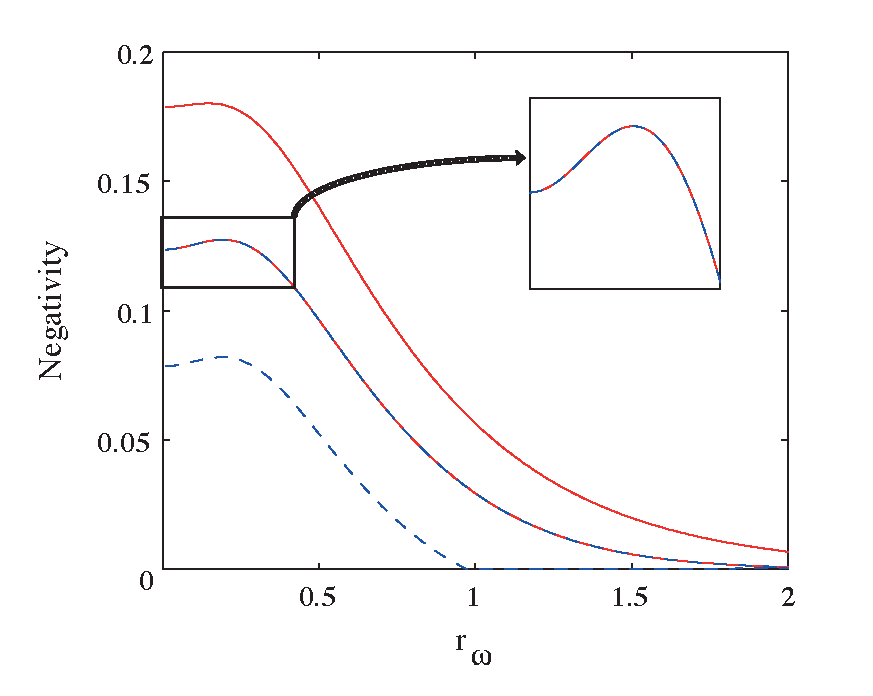
\includegraphics[width=.85\textwidth]{figcdv5bos}
\end{center}
\caption{Entanglement creation for the bosonic scalar field. Negativity for $AR$ (red continuous) and $A\bar R$ (blue dashed) as a function of $r_\omega$ for $\qr=0.85$ and $\qr=1/\sqrt{2}$ (where both contributions are equal). The state considered is of the general form \eqref{geGras}, with $P=0.4$, $\alpha=0$, $\beta=1$.}
\label{ent2}
\end{figure}
\begin{figure}[h]
\begin{center} 
\includegraphics[width=.85\textwidth]{diverg}
\end{center}
\caption{Relative (blue continuous) and absolute (red dashed) entanglement creation  as a function of the inertial negativity for a Grassmann field  state of the family \eqref{geGras} with $P=0.4$, $\beta=0.8$ and different values of $\alpha$ for $\qr=1/\sqrt{2}$ and  $r_\omega=0.15$ (accelerations from $a\approx 5\cdot10^{13}g $ to $5\cdot10^{16} g$ for frequencies from $1 \text{ MHz}$ to $1 \text{ GHz}$). Notice an unbounded growth of the `signal-to-background' ratio.}
\label{unbo}
\end{figure}

We obtain huge `signal-to-background' ratios and the better the negativity can be experimentally determined the bigger this ratio can become. If we relied on entanglement degradation to detect the Unruh effect \cite{Alicefalls}, the percental change in negativity would be bounded by 100 \%. With the plethora of new states presented in this work, this relative change can be made arbitrarily high.


The same analysis carried out for Unruh modes can be repeated if we consider that the excitations $\ket{1}$ are Gaussian wavepackets from the inertial perspective. As detailedly shown in section \ref{sec:peaking}, Gaussian wavepackets of Minkowski modes transform into Gaussian wavepackets of Rindler modes. We can consider at the same time peaked wavepackets in the Minkowskian basis and in the Rindler basis such that the analysis would be completely analogous to the monochromatic case. In this case different choices of $q_\text{R}$ and $q_\text{L}$ represent different spatial/momentum localisation of the Gaussian wavepackets. This means that in principle we can define two local bases (for Alice and Rob) in which this entanglement creation phenomenon is present.


\section{Discussion}

We have shown that the Unruh effect can not only degrade quantum entanglement but also amplify it, banishing previous fundamental misconceptions such as the belief that the Unruh and Hawking effects are sources of entanglement degradation. We have demonstrated that there are families of states whose entanglement can be increased by an arbitrarily high relative factor.

 One could ask why entanglement seems to be created in this case when the natural way of thinking may suggest that under partial tracing correlations can only be lost. This has to do with a mechanism related to the change of basis Unruh-Rindler.  Observing an entangled state of the field from the perspective of an accelerated observer implies two processes: 1) a generation of entanglement due to the Bogoliubov relationships implied in the change of basis that was shadowed under the SMA and 2) an erasure of correlations due to the tracing over one of the Rindler regions. We saw that going beyond the single mode approximation these competing trends explain why for a certain acceleration the amplification of entanglement is maximal. In previous works under the SMA it was simply not possible to see these two mechanisms in action.


Furthermore, with these results we move the experimental difficulties from generating and sustaining high accelerations to the preparation and measurement of quasi-separable entangled states. Hence, we are presenting a new way to detect the Unruh effect. As a matter of fact, our results are independent of the specific implementation to detect the entanglement magnification,  hence they can be exported to a huge variety of experimental set-ups as for instance analog gravity settings.


Besides, these results can be readily exported to a setting consisting in an observer hovering at certain distance close to the event horizon of an Schwarzschild black hole, following chapter \ref{blackhole1}, and therefore the same conclusions drawn for the Unruh effect are also valid for the Hawking effect.




